\captionsetup[subfigure]{justification=justified,singlelinecheck=false}

\begin{figure*}[p]
  \vfill
  \begin{subfigure}[t]{\linewidth}
    \caption{Computational overhead for \mnist \MNISTNET (GPU)}
    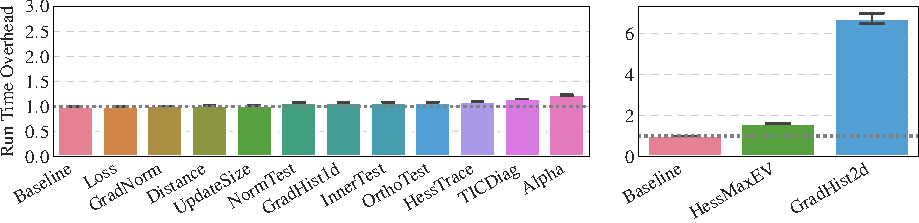
\includegraphics{../repos/cockpit-paper/fig/01_benchmark/output/fig_individual/benchmark_combined_mnist_logreg_cuda_thesis-wide}
    \label{cockpit::fig:app_benchmark_instruments_cuda-mnist_logreg}
  \end{subfigure}
  \vfill
  \begin{subfigure}[t]{\linewidth}
    \caption{Computational overhead for \mnist \mlp (GPU)}
    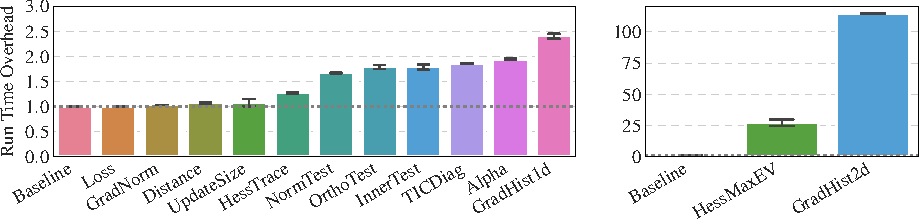
\includegraphics{../repos/cockpit-paper/fig/01_benchmark/output/fig_individual/benchmark_combined_mnist_mlp_cuda_thesis-wide}
    \label{cockpit::fig:app_benchmark_instruments_cuda-mnist_mlp}
  \end{subfigure}
  \vfill
  \begin{subfigure}[t]{\linewidth}
    \caption{Computational overhead for \cifarten \threecthreed (GPU)}
    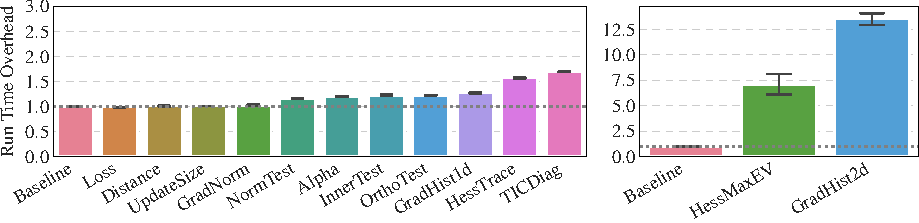
\includegraphics{../repos/cockpit-paper/fig/01_benchmark/output/fig_individual/benchmark_combined_cifar10_3c3d_cuda_thesis-wide}
    \label{cockpit::fig:app_benchmark_instruments_cuda-cifar10}
  \end{subfigure}
  \vfill
  \begin{subfigure}[t]{\linewidth}
    \caption{Computational overhead for \fmnist \twoctwod (GPU)}
    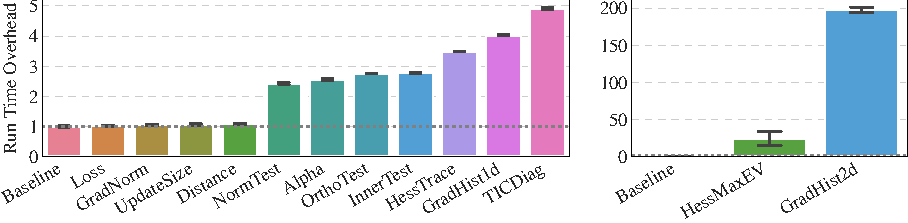
\includegraphics{../repos/cockpit-paper/fig/01_benchmark/output/fig_individual/benchmark_combined_fmnist_2c2d_cuda_thesis-wide}
    \label{cockpit::fig:app_benchmark_instruments_cuda-fmnist}
  \end{subfigure}
  \vfill
  \caption{\textbf{Individual overhead of \cockpittitle's instruments on GPU for
      four different problems.} All run times are shown as multiples of the
    \emph{baseline} without tracking. Expensive quantities are displayed in
    separate panels on the right. Experimental details in the text.}
  \label{cockpit::fig:app_benchmark_instruments_cuda}
\end{figure*}

\captionsetup[subfigure]{justification=centering, singlelinecheck=true}

%%% Local Variables:
%%% mode: latex
%%% TeX-master: "../../../thesis"
%%% End:
